A árvore de decisão, é um mecanismo que permite entendermos uma variável,
estimando seu valor baseado numa regressão, na qual o espaço é subdividido
em duas partes a cada nível. Presta-se assim, a uma caracterização
binária da amostra de dados de entrada.


\section{Árvore gerada}

Utilizando o seed 5668 os dados foram separados em duas amostras aleatórias
de 12500 observações cada.

Através do método CART foi gerada a seguinte árvore com a amostra
de aprendizado:

\begin{center}
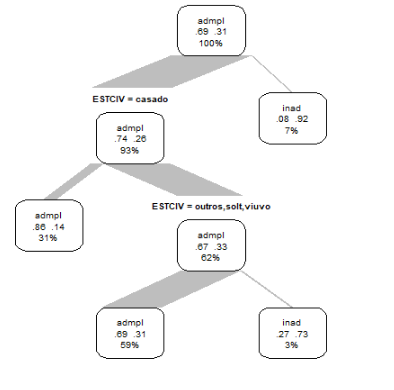
\includegraphics[width=0.9\textwidth]{CartTree}
\par\end{center}

É possível notar que as variáveis mais significantes para a classificação
foram Natureza e Estado Civil. 

\begin{minted}{R}
> printcp(ac1)
\end{minted}

\begin{lstlisting}
Classification tree:
rpart(formula = STATUS ~ UF + ESCOLARIDADE + ESTCIV + FAIXARENDA + 
    NATUREZA, data = calvo.lrn)
 
Variables actually used in tree construction:
[1] ESTCIV   NATUREZA
 
Root node error: 3861/12500 = 0.30888
 
n= 12500 
 
        CP nsplit rel error  xerror     xstd
1 0.182595      0   1.00000 1.00000 0.013379
2 0.018778      1   0.81740 0.81740 0.012580
3 0.010000      3   0.77985 0.77985 0.012383
\end{lstlisting}


Através dos valores CP é possível verificar que os erros para a amostra
de aprendizado foram de 31\% e a menor taxa de erro se encontra no
nó 3 com 78\%, portando não é necessário podar a árvore. 


\section{Validação com Amostra Teste}

\begin{minted}{R}
> CrossTable(calvo.tst$STATUS, yhat_tst, prop.chisq = F, prop.t = F, digits = 2)
\end{minted}

\begin{lstlisting}
   Cell Contents
|-------------------------|
|                       N |
|           N / Row Total |
|           N / Col Total |
|-------------------------|
 
 
Total Observations in Table:  12500 
 
 
                 | yhat_tst 
calvo.tst$STATUS |     admpl |      inad | Row Total | 
-----------------|-----------|-----------|-----------|
           admpl |      8534 |       163 |      8697 | 
                 |      0.98 |      0.02 |      0.70 | 
                 |      0.75 |      0.15 |           | 
-----------------|-----------|-----------|-----------|
            inad |      2869 |       934 |      3803 | 
                 |      0.75 |      0.25 |      0.30 | 
                 |      0.25 |      0.85 |           | 
-----------------|-----------|-----------|-----------|
    Column Total |     11403 |      1097 |     12500 | 
                 |      0.91 |      0.09 |           | 
-----------------|-----------|-----------|-----------|
\end{lstlisting}


Pode-se notar que existe 20\% de erro na amostra de teste, sendo maior
na classificação de adimplentes para inadimplentes (25\%). 
